\chapter{Trường yếu, sóng hấp dẫn và nguyên lý tác dụng}

Các phương trình chính xác của thuyết tương đối rộng là phi tuyến, và dạng theo thành phần của chúng có thể trở nên rất phức tạp ngay cả trước khi ta giải được một bài toán vật lý nào. Trong bài giảng cuối của khóa học, tốt hơn là tách nguyên lý ra khỏi phần kỹ thuật tính toán. Ta sẽ hỏi các phương trình Einstein trở thành gì khi trường hấp dẫn yếu, nhận diện các sóng chứa trong phép gần đúng đó, rồi kết thúc bằng cách thấy các phương trình trường đầy đủ nằm gọn trong một nguyên lý tác dụng cô đọng đến mức đáng kinh ngạc.

Ba câu hỏi dẫn dắt cuộc thảo luận. Trường hấp dẫn yếu nghĩa là gì? Vì sao lý thuyết yếu lại tuyến tính mặc dù lý thuyết chính xác thì không? Và những hiệu ứng vật lý nào phân biệt một sóng hấp dẫn với một sự nhấp nhô đơn thuần của tọa độ?

\section{Một nhiễu loạn nhỏ của hình học cân bằng}

Tính yếu là một lược đồ gần đúng. Nếu một nhiễu loạn không thứ nguyên có cỡ \(\epsilon\ll1\), thì bình phương của nó có cỡ \(\epsilon^2\), và một phép tính bậc nhất sẽ nhất quán bỏ qua hạng sau. Ví dụ quen thuộc là một hệ cơ học dao động nhỏ quanh vị trí cân bằng. Các phương trình chính xác của nó có thể phi tuyến, nhưng các dao động đủ nhỏ thì tuân theo các phương trình tuyến tính.

Đối với hấp dẫn, nền cân bằng sẽ là không-thời gian phẳng rỗng. Bắt đầu với phương trình chân không của Einstein,
\begin{equation}
 R_{\mu\nu}-\frac12 g_{\mu\nu}R=0.
 \label{eq:l10-vacuum-einstein}
\end{equation}
Lấy vết của nó trong bốn chiều cho
\begin{equation}
 g^{\mu\nu}
 \left(R_{\mu\nu}-\frac12 g_{\mu\nu}R\right)
 =R-2R=-R=0,
\end{equation}
vì vậy phương trình chân không tương đương với
\begin{equation}
 R_{\mu\nu}=0.
 \label{eq:l10-ricci-flat}
\end{equation}

\begin{figure}[htbp]
\centering
\includegraphics[width=0.68\textwidth]{lecture_10_figure_02.png}
\caption{Phương trình chân không \(R_{\mu\nu}=0\), được tách riêng ra ở phần đầu của lập luận trường yếu.}
\lectureframe{00:03:11}
\end{figure}

Ở đây, cân bằng có nghĩa là một nghiệm không nguồn và không phụ thuộc thời gian. Không-thời gian phẳng là nghiệm đơn giản nhất như vậy. Có một điểm lưu ý thiết yếu: tính phẳng không có nghĩa là các thành phần của metric bằng một ma trận nhất định trong mọi hệ tọa độ. Nó có nghĩa là có thể chọn các tọa độ quán tính sao cho
\begin{equation}
 g_{\mu\nu}=\eta_{\mu\nu}.
\end{equation}
Sự phân biệt giữa hình học và các tọa độ dùng để mô tả nó sẽ sớm trở thành điểm tinh tế trung tâm.

Bây giờ hãy tưởng tượng một nguồn dữ dội như một hệ nhị phân cô đặc. Trường gần của nó có thể mạnh, nhưng xa nguồn thì nhiễu loạn lan ra và trở nên nhỏ. Khi đó, trong một hệ tọa độ thích hợp, metric có thể được viết
\begin{equation}
 g_{\mu\nu}(x)=\eta_{\mu\nu}+h_{\mu\nu}(x),
 \qquad |h_{\mu\nu}|\ll1.
 \label{eq:weak-split}
\end{equation}
Nhiễu loạn \(h_{\mu\nu}\) được phép phụ thuộc vào cả bốn tọa độ không-thời gian. Tính yếu có nghĩa là các lũy thừa cao hơn bậc nhất sẽ bị bỏ qua.

\section{Những gì còn lại ở bậc nhất}

Biểu thức đầy đủ của tensor Ricci quá dài nên ở giai đoạn này không hữu ích. Chỉ cần cấu trúc của nó là đủ. Các ký hiệu Christoffel chứa một metric nghịch đảo và một đạo hàm của metric, còn độ cong thì chứa một đạo hàm của một ký hiệu Christoffel và tích của hai ký hiệu Christoffel:
\begin{equation}
 \Gamma\sim\frac12 g^{-1}\partial g,
 \qquad
 R\sim\partial\Gamma+\Gamma\Gamma.
 \label{eq:curvature-skeleton}
\end{equation}

\begin{figure}[htbp]
\centering
\includegraphics[width=0.84\textwidth]{lecture_10_figure_03.png}
\caption{Phép tách trường yếu và cách dựng sơ đồ \(R\sim\partial\Gamma+\Gamma\Gamma\). Ký hiệu này bộc lộ các bậc theo \(h\) mà không cần khai triển mọi chỉ số.}
\lectureframe{00:10:17}
\end{figure}

Metric nghịch đảo suy ra từ
\(g^{\mu\alpha}g_{\alpha\nu}=\delta^\mu{}_\nu\). Ở bậc nhất,
\begin{equation}
 g^{\mu\nu}=\eta^{\mu\nu}-h^{\mu\nu}+O(h^2),
 \label{eq:inverse-weak}
\end{equation}
trong đó các chỉ số của \(h\) được nâng bằng metric nền. Trong các tọa độ quán tính, nền là hằng số,
\begin{equation}
 \partial_\alpha\eta_{\mu\nu}=0,
\end{equation}
và do đó
\begin{equation}
 \partial_\alpha g_{\mu\nu}
 =\partial_\alpha h_{\mu\nu}.
\end{equation}
Hệ quả là,
\begin{equation}
\begin{aligned}
 \Gamma&=O(\partial h),\\
 R_{\mu\nu}
 &=O(\partial\partial h)+O\bigl((\partial h)^2\bigr)\\
 &\quad+O(h\,\partial\partial h).
\end{aligned}
 \label{eq:ricci-orders}
\end{equation}

\begin{figure}[htbp]
\centering
\includegraphics[width=0.84\textwidth]{lecture_10_figure_04.png}
\caption{Phép khai triển trên bảng của metric nghịch đảo và nhận xét rằng \(\partial\eta=0\). Ở bậc dẫn đầu, chỉ còn lại các đạo hàm của \(h_{\mu\nu}\).}
\lectureframe{00:11:55}
\end{figure}

Hai hạng cuối trong Phương trình~\eqref{eq:ricci-orders} là bậc hai theo nhiễu loạn nên bị lược bỏ. Vì thế, các phương trình chân không là các phương trình tuyến tính chứa các đạo hàm bậc hai của \(h_{\mu\nu}\). Đó chính là toàn bộ ý nghĩa của việc tuyến tính hóa. Điều này không khẳng định rằng lý thuyết chính xác của Einstein là tuyến tính.

\begin{classroomqa}
\audiencequestion{Tensor độ cong có 4 chỉ số, còn tensor Ricci có 2. Nếu hai đạo hàm đã mang chỉ số và \(h_{\mu\nu}\) lại mang thêm 2 chỉ số nữa, thì việc đếm chỉ số diễn ra thế nào?}
\lecturerresponse{Tensor Ricci thu được bằng cách co một cặp chỉ số trong tensor độ cong. Metric được dùng trong phép co đó để lại 2 chỉ số tự do, đúng là cặp chỉ số mà \(R_{\mu\nu}\) mang. Dạng ký hiệu \(\partial\partial h\) lược bỏ các phép co ấy; đó là phép đếm bậc, không phải một công thức đầy đủ có chỉ số.
\lecturetimestamp{00:18:45--00:19:53}}
\end{classroomqa}

\begin{classroomqa}
\audiencequestion{Việc co với metric nghịch đảo có đưa vào những hạng như \(h\,\partial^2h\) hay không, và nếu có thì vì sao có thể bỏ qua chúng?}
\lecturerresponse{Có. Thay \(g^{-1}\) bằng
\(\eta^{-1}-h+\cdots\) tạo ra vừa hạng tuyến tính
\(\eta^{-1}\partial^2h\) vừa các hiệu chỉnh chứa thêm một \(h\). Các hạng sau là bậc hai. Cùng quy tắc ấy loại bỏ
\(h\,\partial h\), \(h\,\partial^2h\) và
\((\partial h)^2\). Chỉ giữ lại một lũy thừa của nhiễu loạn chính là đúng phép gần đúng đang được thực hiện.
\lecturetimestamp{00:19:55--00:21:14}}
\end{classroomqa}

\section{Vì sao các phương trình có dạng sóng}

Các phương trình trường bậc hai theo đạo hàm tự nhiên gợi ra sự lan truyền sóng. Đối với một hàm vô hướng lan truyền dọc theo trục \(z\), dạng mẫu là
\begin{equation}
 \left(\partial_t^2-\partial_z^2\right)\phi=0,
\end{equation}
mà các nghiệm của nó bao gồm các biên dạng truyền sang phải và sang trái tùy ý,
\begin{equation}
 \phi(z,t)=f(z-t)+g(z+t).
\end{equation}
Trong 3 chiều không gian, cùng phương trình đó là
\begin{equation}
 \left(\partial_t^2-\nabla^2\right)\phi=0.
\end{equation}
Tính tuyến tính của nó cho phép nguyên lý chồng chất: tổng của hai nghiệm lại là một nghiệm khác.

Hấp dẫn không phải là một trường vô hướng. Nhiễu loạn có các thành phần tensor, và thoạt đầu phương trình \(R_{\mu\nu}=0\) dường như cung cấp nhiều phương trình theo thành phần. Không phải tất cả chúng đều độc lập; một số là các ràng buộc và một số phản ánh tự do tọa độ. Sự tương tự ở đây là với lý thuyết Maxwell, nơi một hệ các phương trình trường rốt cuộc chỉ còn lại các sóng ngang vật lý.

Sau khi áp đặt các điều kiện tọa độ thích hợp, các thành phần bức xạ tuân theo một phương trình sóng thông thường,
\begin{equation}
 \Box h_{\mu\nu}=0,
 \qquad
 \Box=\eta^{\alpha\beta}\partial_\alpha\partial_\beta.
 \label{eq:linear-wave}
\end{equation}
Các dấu cụ thể bên trong \(\Box\) phụ thuộc vào quy ước chữ ký; nội dung của nó thì không. Các nhiễu loạn lan truyền trên nón ánh sáng.

\section{Những nhấp nhô của tọa độ không phải là sóng hấp dẫn}

Trước khi chấp nhận mọi nghiệm của các phương trình đã tuyến tính hóa là một sóng vật lý, ta phải trở lại lưu ý về tọa độ. Không gian phẳng có thể được mô tả bằng các đường tọa độ cong. Khi đó, các thành phần metric của nó khác các giá trị trong hệ Cartesian dù độ cong của nó vẫn bằng 0.

Chính tấm bảng cung cấp ví dụ này. Hãy vẽ các tọa độ Cartesian thẳng trên bề mặt phẳng của nó và viết
\begin{equation}
 ds^2=\delta_{mn}\,dx'^m dx'^n.
\end{equation}
Bây giờ gán nhãn lại chính những điểm ấy bằng các tọa độ hơi nhấp nhô,
\begin{equation}
 x'^m=x^m+f^m(x).
 \label{eq:small-coordinate-change}
\end{equation}
Các vi phân trở thành
\begin{equation}
 dx'^m=dx^m+\partial_n f^m\,dx^n.
\end{equation}
Thế vào phần tử độ dài và chỉ giữ đến bậc nhất theo \(f\) cho
\begin{align}
 ds^2
 &=\delta_{mn}dx^m dx^n\\
 &\quad+\left(\partial_m f_n+\partial_n f_m\right)dx^m dx^n
 +O(f^2).
\end{align}
Vì vậy, một nhiễu loạn có vẻ như có dạng
\begin{equation}
 h_{mn}=\partial_m f_n+\partial_n f_m
 \label{eq:pure-gauge}
\end{equation}
thực ra hoàn toàn không mô tả hình học mới nào. Nó là không gian phẳng trong các tọa độ nhấp nhô.

\begin{figure}[htbp]
\centering
\includegraphics[width=0.84\textwidth]{lecture_10_figure_05.png}
\caption{Phép tính về sự nhấp nhô tọa độ trên bảng. Một phép đổi tọa độ nhỏ tạo ra một \(h_{mn}\) có vẻ nhỏ mặc dù tấm bảng vẫn phẳng.}
\lectureframe{00:27:54}
\end{figure}

Phương trình~\eqref{eq:pure-gauge} là dạng tuyến tính hóa của tự do tọa độ, hay tự do chuẩn. Cần thêm các điều kiện bổ sung để khử những nhiễu loạn giả này. Đại số chuẩn chi tiết không được triển khai ở đây. Vai trò của nó mới là điểm quan trọng: nó loại bỏ những thay đổi trong cách mô tả đồng thời vẫn giữ lại những thay đổi của độ cong. Một khi đã xét đến tự do tọa độ và các phương trình ràng buộc, nội dung vật lý còn lại quy về 2 phân cực sóng độc lập.

\begin{figure}[htbp]
\centering
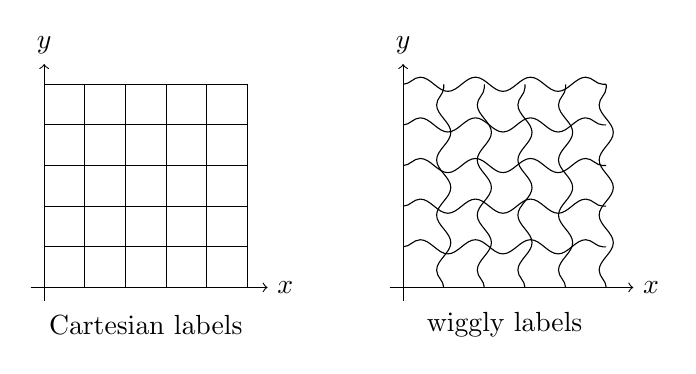
\begin{tikzpicture}[scale=0.86]
\begin{scope}
\draw[->] (-0.2,0) -- (3.3,0) node[right] {$x$};
\draw[->] (0,-0.2) -- (0,3.3) node[above] {$y$};
\foreach \u in {0.6,1.2,1.8,2.4,3.0}{
  \draw (\u,0) -- (\u,3.0);
  \draw (0,\u) -- (3.0,\u);
}
\node at (1.5,-0.55) {Cartesian labels};
\end{scope}
\begin{scope}[xshift=5.3cm]
\draw[->] (-0.2,0) -- (3.4,0) node[right] {$x$};
\draw[->] (0,-0.2) -- (0,3.3) node[above] {$y$};
\foreach \u in {0.6,1.2,1.8,2.4,3.0}{
  \draw[decorate,decoration={snake,amplitude=0.09cm,segment length=0.7cm}]
    (\u,0) -- (\u,3.0);
  \draw[decorate,decoration={snake,amplitude=0.09cm,segment length=0.7cm}]
    (0,\u) -- (3.0,\u);
}
\node at (1.5,-0.55) {wiggly labels};
\end{scope}
\end{tikzpicture}
\caption{Hình học vẫn phẳng trong khi lưới tọa độ thay đổi. Chỉ riêng các thành phần metric không thể quyết định liệu một nhiễu loạn có phải là vật lý hay không.}
\end{figure}

\section{Một sóng truyền dọc theo trục z}

Hãy chọn một sóng phẳng truyền theo chiều dương của trục \(z\). Pha của nó có thể được viết
\begin{equation}
 k(z-t),
\end{equation}
nên một thành phần tiêu biểu có dạng
\begin{equation}
 h_{\mu\nu}(z,t)
 =h_{\mu\nu}^{(0)}\sin k(z-t).
 \label{eq:plane-wave}
\end{equation}
Các mặt pha không đổi thỏa mãn \(z-t=\text{constant}\); do đó tốc độ lan truyền là tốc độ ánh sáng.

Trong mô tả ngang-không vết, các thành phần chứa một chỉ số thời gian hoặc một chỉ số \(z\) đều triệt tiêu:
\begin{equation}
 h_{0\mu}=0,
 \qquad
 h_{z\mu}=0.
 \label{eq:tt-transverse}
\end{equation}
Chỉ còn lại khối \(x\)-\(y\). Nó đối xứng và không vết,
\begin{equation}
 h_{xy}=h_{yx},
 \qquad
 h_{xx}+h_{yy}=0.
 \label{eq:tt-trace}
\end{equation}

\begin{figure}[htbp]
\centering
\includegraphics[width=0.84\textwidth]{lecture_10_figure_06.png}
\caption{Một sóng truyền dọc theo \(z\), được biểu diễn như một chồng các mặt phẳng ngang. Các biên độ \(x\)-\(y\) còn lại tuân theo \(h_{xx}+h_{yy}=0\).}
\lectureframe{00:43:36}
\end{figure}

Do đó có 2 kiểu độc lập. Với
\(i,j\in\{x,y\}\), chúng có thể được biểu diễn dưới dạng
\begin{equation}
 h^{\mathrm{TT}}_{ij}(z,t)
 =
 \begin{pmatrix}
 h_+ & h_\times\\
 h_\times & -h_+
 \end{pmatrix}
 \sin k(z-t).
 \label{eq:polarization-matrix}
\end{equation}
Kiểu đường chéo được gọi là phân cực cộng. Kiểu ngoài đường chéo được gọi là phân cực chéo. Quay các trục ngang đi \(45^\circ\) sẽ biến kiểu này thành kiểu kia, và một sóng phân cực tuyến tính bất kỳ là chồng chất của cả hai. Trong lý thuyết này không có thêm phân cực độc lập nào khác.

\begin{figure}[htbp]
\centering
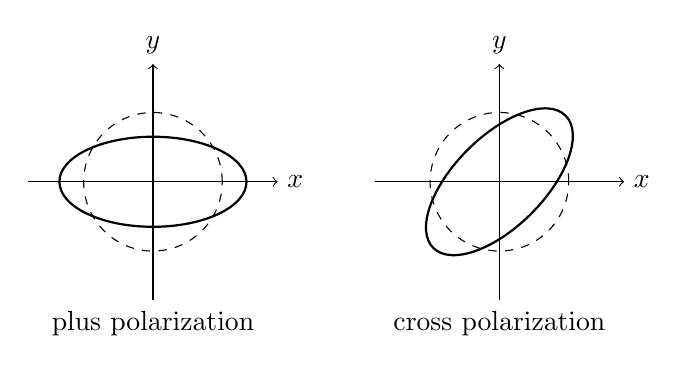
\begin{tikzpicture}[scale=0.88]
\begin{scope}
\draw[->] (-1.8,0) -- (1.8,0) node[right] {$x$};
\draw[->] (0,-1.7) -- (0,1.7) node[above] {$y$};
\draw[dashed] (0,0) circle (1.0);
\draw[thick] (0,0) ellipse (1.35 and 0.65);
\node at (0,-2.05) {plus polarization};
\end{scope}
\begin{scope}[xshift=5.0cm]
\draw[->] (-1.8,0) -- (1.8,0) node[right] {$x$};
\draw[->] (0,-1.7) -- (0,1.7) node[above] {$y$};
\draw[dashed] (0,0) circle (1.0);
\draw[thick,rotate=45] (0,0) ellipse (1.35 and 0.65);
\node at (0,-2.05) {cross polarization};
\end{scope}
\end{tikzpicture}
\caption{Trong nửa chu kỳ, một phương ngang bị kéo giãn còn phương vuông góc bị nén lại. Sau nửa chu kỳ nữa, biến dạng đảo chiều.}
\end{figure}

\section{Từ các thành phần metric đến độ biến dạng vật lý}

Giữ cố định \(z\) và \(t\) rồi khảo sát mặt phẳng ngang. Đối với một sóng phân cực cộng thuần,
\begin{equation}
 ds_\perp^2
 =(1+h_{xx})\,dx^2+(1-h_{xx})\,dy^2.
 \label{eq:transverse-distance}
\end{equation}
Khi \(h_{xx}>0\), một khoảng tọa độ cố định theo hướng \(x\) có độ dài riêng hơi lớn hơn, trong khi khoảng tương ứng theo \(y\) có độ dài riêng hơi nhỏ hơn. Nửa chu kỳ sau, \(h_{xx}\) đổi dấu, và vai trò đảo ngược. Một hình vuông luân phiên bị kéo giãn theo phương ngang và nén theo phương thẳng đứng, rồi bị nén theo phương ngang và kéo giãn theo phương thẳng đứng. Đối với phân cực chéo, sự luân phiên tương tự xảy ra dọc theo các trục quay đi \(45^\circ\).

Đến bậc nhất, một nhánh ban đầu có độ dài \(L\) biến đổi theo
\begin{equation}
 \frac{\Delta L}{L}\simeq\frac12 h_{ij}n^i n^j,
 \label{eq:fractional-strain}
\end{equation}
trong đó \(\mathbf n\) chỉ dọc theo nhánh. Công thức này chuyển nhiễu loạn metric thành độ biến dạng không thứ nguyên mà một bộ dò đo được.

\begin{classroomqa}
\audiencequestion{Một thước mét được giữ gắn kết bằng tương tác điện từ và không đơn thuần thay đổi độ dài nghỉ theo các tọa độ. Vậy trong hình minh họa có nên dùng các khối lượng thử tự do tách rời thay vào đó không?}
\lecturerresponse{Sự phân biệt ấy rất quan trọng. Một thanh thực có tính đàn hồi, nên trường thủy triều gây ra ứng suất bên trong nó; một thanh thép và một thanh gỗ nói chung sẽ đáp ứng với những mức độ khác nhau. Các khối lượng thử treo tự do tránh được chính đáp ứng đàn hồi đó và cho thấy gia tốc tương đối trực tiếp hơn. Trong cả hai trường hợp, sóng đi qua không chỉ đơn thuần là việc gán nhãn lại các điểm. Độ cong phụ thuộc thời gian của nó tạo ra một hiệu ứng vật lý.
\lecturetimestamp{00:47:23--00:48:48}}
\end{classroomqa}

Phát biểu cục bộ chính xác là sự lệch trắc địa. Với các hạt rơi tự do ở gần nhau, cách nhau bởi \(\xi^i\),
\begin{equation}
 \frac{d^2\xi^i}{dt^2}
 =-R^i{}_{0j0}\,\xi^j.
 \label{eq:geodesic-deviation}
\end{equation}
Trong sóng ngang-không vết yếu,
\begin{equation}
 R_{0i0j}=-\frac12\ddot h^{\mathrm{TT}}_{ij},
 \label{eq:tidal-curvature}
\end{equation}
nên metric dao động sinh ra gia tốc thủy triều luân phiên. Đó là lý do vì sao không thể gạt một sóng phụ thuộc thời gian đi như chỉ là một cách chọn thước đo tĩnh. Nó có độ cong khác không.

\begin{classroomqa}
\audiencequestion{Nếu mọi thước đo trong vùng đều bị ảnh hưởng, thì cái gì có thể đo được sự nén và kéo giãn?}
\lecturerresponse{Một cảm biến biến dạng có thể ghi nhận ứng suất thật sự được cảm ứng trong một vật thể vật chất. Tốt hơn nữa, người ta có thể theo dõi khoảng cách thay đổi giữa các khối lượng treo tự do. Một phép co giãn lại tĩnh, đồng đều có thể bị hấp thụ vào thiết bị đo, nhưng độ cong dao động gây ra một đáp ứng có thể được ghi lại.
\lecturetimestamp{00:51:10--00:52:02}}
\end{classroomqa}

\section{Nguồn và bộ dò}

Sóng điện từ được tạo ra bởi các điện tích và dòng điện chuyển động. Sóng hấp dẫn được tạo ra bởi các phân bố khối lượng và năng lượng chuyển động. Bảo toàn năng lượng và động lượng loại trừ bức xạ hấp dẫn đơn cực và lưỡng cực đối với một hệ cô lập, nên mômen bức xạ dẫn đầu là tứ cực. Một hệ nhị phân đặc chắc cung cấp đúng mômen tứ cực biến thiên cần thiết: hai vật thể đậm đặc quay quanh nhau và phát sóng vào vùng trường xa.

Ở gần hệ nhị phân, không-thời gian cong mạnh và khai triển tuyến tính của Phương trình~\eqref{eq:weak-split} không đáng tin cậy. Ở xa, sóng phát ra lan trên một diện tích lớn hơn, biên độ của nó trở nên nhỏ, và mô tả tuyến tính hóa trở nên chính xác. Đối với một người quan sát nằm trên trục \(z\) tính từ nguồn, sự kéo giãn đo được nằm trong mặt phẳng ngang \(x\)-\(y\).

\begin{classroomqa}
\audiencequestion{Thước trong hình vẽ là một thước tọa độ trừu tượng hay một thước mét vật lý, và làm sao một thước có độ dài biến đổi lại có thể đo được hiệu ứng ấy?}
\lecturerresponse{Nó có thể là một vật thể vật lý, nhưng khi đó các tính chất vật liệu của nó trở nên quan trọng. Độ cong cung cấp ứng suất thủy triều; thép và gỗ không nhất thiết biến dạng giống hệt nhau dưới tác dụng đó. So sánh đáp ứng của chúng đã là một phép đo. Một bộ dò sạch hơn thay các thanh bằng các khối lượng thử tách rời và đo chuyển động vi sai của chúng.
\lecturetimestamp{00:54:00--00:55:19}}
\end{classroomqa}

Một chiến lược là dùng bộ dò cộng hưởng. Nếu một hệ cơ học có tần số riêng gần với tần số của sóng tới, sóng sẽ kích thích nó một cách kết hợp pha và khuếch đại đáp ứng. Một giao thoa kế dùng một chiến lược khác: các gương đóng vai trò các khối lượng thử, và giao thoa laser so sánh độ dài hiệu dụng của hai nhánh vuông góc. Một sóng phân cực cộng làm dài một nhánh đồng thời rút ngắn nhánh kia, đúng bằng tín hiệu vi sai mà giao thoa kế được thiết kế để phát hiện.

\begin{classroomqa}
\audiencequestion{Đây có phải là cơ sở của một bộ dò sóng hấp dẫn không?}
\lecturerresponse{Đúng. Một thanh cứng hầu như không thay đổi, trong khi các khối lượng ở đầu mút treo tự do có thể chịu gia tốc tương đối. Người ta cũng có thể khai thác cộng hưởng để một lực kích thích tuần hoàn yếu tạo ra đáp ứng lớn hơn. Độ biến dạng thiên văn dự kiến là cực kỳ nhỏ, cỡ \(10^{-21}\), vì vậy thiết kế bộ dò là nghệ thuật biến chuyển động vi sai cực nhỏ đó thành một tín hiệu đo được.
\lecturetimestamp{00:55:20--00:57:10}}
\end{classroomqa}

\begin{classroomqa}
\audiencequestion{LIGO có phải là một ví dụ của kiểu bộ dò như vậy không?}
\lecturerresponse{Đúng. Các đại lượng quan sát cơ bản của nó xuất phát từ ánh sáng laser phản xạ giữa các gương trong hai nhánh vuông góc. Sóng hấp dẫn làm thay đổi các độ dài quang lộ tương đối và do đó làm thay đổi hình giao thoa. Vào thời điểm của bài giảng này, thiết bị ấy vẫn chưa có một phép phát hiện trực tiếp; về sau tình hình lịch sử đó đã thay đổi.\editorialnote{Quan sát trực tiếp đầu tiên, GW150914, được ghi nhận vào 2015 và được công bố vào 2016.}
\lecturetimestamp{00:57:16--00:58:05}}
\end{classroomqa}

\begin{classroomqa}
\audiencequestion{Từ nghiệm sóng suy ra tốc độ lan truyền nào?}
\lecturerresponse{Tốc độ ánh sáng. Pha \(k(z-t)\) dịch chuyển một đơn vị theo \(z\) trong một đơn vị theo \(t\), và phương trình Einstein tuyến tính hóa có cùng cấu trúc lan truyền theo nón ánh sáng như phương trình sóng điện từ.
\lecturetimestamp{00:58:07--00:58:16}}
\end{classroomqa}

Va chạm hố đen và các hệ nhị phân đặc chắc là những nguồn đặc biệt hứa hẹn. Gần va chạm, trường hấp dẫn phi tuyến dữ dội, và một phần đáng kể năng lượng được giải phóng có thể thoát đi dưới dạng bức xạ hấp dẫn. Đến khi tín hiệu tới được một bộ dò ở xa, biên độ của nó đã đủ yếu để sự lan truyền sóng tuyến tính là một mô tả rất tốt. Vì thế bức xạ hấp dẫn mở ra một kênh thiên văn không nhất thiết phải phụ thuộc vào ánh sáng phát ra.

\section{Pulsar nhị phân và bằng chứng gián tiếp}

Bức xạ mang năng lượng. Nếu một hệ nhị phân phát ra sóng hấp dẫn, năng lượng quỹ đạo giảm đi, các vật thể từ từ xoắn ốc vào trong, và chu kỳ quỹ đạo thay đổi. Pulsar nhị phân cung cấp một chiếc đồng hồ đủ chính xác để đo sự thay đổi đó. Sự tiến hóa quỹ đạo quan sát được của nó phù hợp về mặt định lượng với mức mất năng lượng do thuyết tương đối rộng dự đoán.

Trong bối cảnh lịch sử của bài giảng, đây là bằng chứng gián tiếp có tính quyết định: chưa có bộ dò nào ghi nhận một sóng đi qua Trái Đất, nhưng quỹ đạo đã mất năng lượng đúng với tốc độ mà bức xạ hấp dẫn đòi hỏi. Sóng đã có thể quan sát được thông qua những gì chúng gây ra cho nguồn của mình.

\begin{classroomqa}
\audiencequestion{Tần số hay chu kỳ nào đặc trưng cho hệ pulsar nhị phân ban đầu? Có phải nó ở thang mili giây không?}
\lecturerresponse{Thang mili giây nói đến sự tự quay của một pulsar, chứ không phải quỹ đạo của hai ngôi sao. Trong lớp, người ta kiểm tra giá trị ấy và thấy một chu kỳ quỹ đạo khoảng \(7.75\) giờ. Sự phân biệt này rất quan trọng: bức xạ hấp dẫn bám theo chuyển động quỹ đạo của hệ nhị phân, còn các xung vô tuyến cung cấp chiếc đồng hồ chính xác dùng để theo dõi nó.
\lecturetimestamp{01:01:27--01:03:28}}
\end{classroomqa}

\begin{classroomqa}
\audiencequestion{Qua nhiều thập kỷ quan sát, độ thay đổi tích lũy trong định thời quỹ đạo lớn đến mức nào?}
\lecturerresponse{Độ dịch lũy tích được nêu ra vào khoảng ba mươi giây. Độ thay đổi phân số tức thời thì rất nhỏ, nhưng nhiều thập kỷ định thời xung chính xác khiến hiệu ứng tích lũy trở nên thấy được.
\lecturetimestamp{01:03:34--01:03:54}}
\end{classroomqa}

\section{Sự phụ thuộc theo thời gian, độ cong và các giới hạn của tính tuyến tính}

\begin{classroomqa}
\audiencequestion{Tại sao lại chọn mặt phẳng ngang \(x\)-\(y\)? Điều gì xảy ra nếu thay vào đó xét một mặt phẳng có \(x\) và \(t\)?}
\lecturerresponse{Bản thân sóng phụ thuộc vào cả \(z\) và \(t\), nhưng ngang ở đây chỉ các phương không gian vuông góc với hướng lan truyền trong không gian của nó. Đối với một sóng truyền dọc theo \(z\), các biên độ metric vật lý có thể được chọn nằm trong khối \(x\)-\(y\). Những thành phần biểu kiến khác hoặc không có, hoặc chỉ là các dao động tọa độ có thể loại bỏ.
\lecturetimestamp{01:02:22--01:03:17}}
\end{classroomqa}

\begin{classroomqa}
\audiencequestion{Bản thân thời gian có dao động không?}
\lecturerresponse{Không. Sóng dao động như một hàm của thời gian. Tại một vị trí không gian cố định, các thành phần \(h_{ij}(z,t)\) biến thiên tuần hoàn. Thời gian là một tọa độ mà trường phụ thuộc vào, chứ không phải một đối tượng đang luân phiên bị kéo giãn và nén trong cách hình dung này.
\lecturetimestamp{01:04:00--01:04:18}}
\end{classroomqa}

\begin{classroomqa}
\audiencequestion{Nếu mọi \(h_{0\mu}\) đều triệt tiêu, có phải không hề có độ cong nào liên quan đến phương thời gian không?}
\lecturerresponse{Vẫn có. Các thành phần không gian còn lại phụ thuộc thời gian, và độ cong chứa hai đạo hàm của chúng. Vì vậy các đạo hàm như \(\partial_t^2h_{ij}\) sinh ra các thành phần \(R_{0i0j}\). Việc các thành phần mang chỉ số thời gian của \(h_{\mu\nu}\) triệt tiêu không kéo theo độ cong phụ thuộc thời gian cũng triệt tiêu.
\lecturetimestamp{01:05:15--01:06:09}}
\end{classroomqa}

Phương trình sóng tuyến tính xuất hiện vì \(h\) được giả sử là nhỏ, chứ không phải vì các tạo tác tọa độ đã được loại bỏ. Đó là hai thao tác tách biệt. Việc cố định chuẩn xác định các bậc tự do vật lý; phép tuyến tính hóa loại bỏ các tương tác phi tuyến.

\begin{classroomqa}
\audiencequestion{Phương trình Einstein là phi tuyến, nhưng phương trình sóng thu được lại là tuyến tính. Tính tuyến tính ấy có phải do việc loại bỏ các nghiệm phi vật lý không?}
\lecturerresponse{Không. Nó là do gần đúng biên độ nhỏ. Các hạng chứa \(h\) ở bậc hai đã bị bỏ đi. Việc loại bỏ các gợn tọa độ quyết định nghiệm nào là vật lý; đó không phải là điều làm cho phương trình trở nên tuyến tính.
\lecturetimestamp{01:06:45--01:07:29}}
\end{classroomqa}

\begin{classroomqa}
\audiencequestion{Sau khi giải phương trình đã tuyến tính hóa, sai số so với một nghiệm chính xác lớn đến mức nào?}
\lecturerresponse{Các hiệu chỉnh đầu tiên bị bỏ qua có bậc \(h^2\). Nếu \(h\sim10^{-1}\) thì chúng có bậc \(10^{-2}\); nếu \(h\sim10^{-3}\) thì chúng có bậc \(10^{-6}\). Một phép tính nhiễu loạn luôn phải được kiểm tra lại sau đó để bảo đảm rằng tham số nhỏ đã giả định thực sự là nhỏ.
\lecturetimestamp{01:07:35--01:08:31}}
\end{classroomqa}

\begin{classroomqa}
\audiencequestion{Khi các hạng bậc cao hơn trở nên quan trọng, sóng có mất đi tính chất ngang không?}
\lecturerresponse{Tính chất bức xạ ngang cốt yếu vẫn còn, nhưng nguyên lý chồng chất tuyến tính thì không. Các sóng mạnh tương tác với trường hấp dẫn do các sóng khác mang theo; thay vì đi xuyên qua nhau mà không đổi, chúng tán xạ.
\lecturetimestamp{01:08:34--01:09:11}}
\end{classroomqa}

\begin{classroomqa}
\audiencequestion{Tốc độ của một sóng cơ học phụ thuộc vào độ cứng và mật độ. Có một nghĩa tương tự nào mà theo đó không-thời gian có độ cứng không?}
\lecturerresponse{Chỉ theo nghĩa loại suy. Đối với một môi trường vật chất, sự lan truyền phụ thuộc vào một tổ hợp như độ cứng chia cho mật độ. Vì sóng điện từ và sóng hấp dẫn lan truyền với \(c\), ngôn ngữ cơ học cũ sẽ gọi môi trường của chúng là cứng một cách phi thường. Vật lý hiện đại không gán cho không-thời gian một môđun Young thông thường; điều bất biến là sự lan truyền với tốc độ ánh sáng do các phương trình trường ấn định.
\lecturetimestamp{01:09:12--01:11:10}}
\end{classroomqa}

\section{Con đường thứ hai: Tác dụng dừng}

Khi phần thảo luận về sóng đã hoàn tất, ta còn thời gian cho một lần thay đổi quan điểm cuối cùng. Nguyên lý tác dụng dừng là ngôn ngữ chung của cơ học cổ điển, điện từ học, lý thuyết trường và Mô hình Chuẩn. Thuyết tương đối rộng thuộc về cùng một cấu trúc.

Đối với một hạt, tác dụng là một tích phân dọc theo một quỹ đạo. Đối với một trường, một lịch sử gán một giá trị trường \(\phi(x)\) cho mọi điểm của không-thời gian, và tác dụng là một tích phân trên không-thời gian:
\begin{equation}
 S[\phi]
 =\int d^4x\,
 \mathcal L\bigl(\phi,\partial_\mu\phi\bigr).
 \label{eq:field-action}
\end{equation}
Mỗi \(\phi(x)\) đủ trơn đều là một lịch sử khả dĩ, cũng như mỗi đường đi đủ trơn đều là một quỹ đạo hạt khả dĩ, nhưng đa số không phải là nghiệm. Các lịch sử vật lý là các điểm dừng của tác dụng với dữ liệu biên được giữ cố định:
\begin{equation}
 \delta S=0.
 \label{eq:stationary-action}
\end{equation}
Đối với một trường, biên bao quanh một miền không-thời gian thay vì chỉ xác định hai đầu mút của một đường đi. Khi đó, các phương trình Euler--Lagrange chọn ra phần nội suy giữa các giá trị biên đã cho.

Các phương trình trường của Einstein có thể được suy ra đúng theo cách này. Phép biến phân thì dài, nhưng bản thân tác dụng lại đơn giản. Trước khi viết nó ra, ta cần độ đo thích hợp của thể tích không-thời gian.

\section{Vì sao định thức đo thể tích}

Bắt đầu trong hai chiều với một metric đường chéo,
\begin{equation}
 ds^2=g_{xx}\,dx^2+g_{yy}\,dy^2.
\end{equation}
Một hình chữ nhật tọa độ có các cạnh \(dx\) và \(dy\) có các độ dài riêng của cạnh là \(\sqrt{g_{xx}}\,dx\) và \(\sqrt{g_{yy}}\,dy\), nên diện tích riêng của nó là
\begin{equation}
 dA
 =\sqrt{g_{xx}g_{yy}}\,dx\,dy.
\end{equation}
Nếu có mặt thành phần ngoài đường chéo \(g_{xy}\), các cạnh tọa độ không nhất thiết vuông góc. Diện tích đã hiệu chỉnh là
\begin{equation}
 dA
 =\sqrt{g_{xx}g_{yy}-g_{xy}^2}\,dx\,dy
 =\sqrt{\det g}\,dx\,dy.
 \label{eq:area-determinant}
\end{equation}

\begin{figure}[htbp]
\centering
\includegraphics[width=0.84\textwidth]{lecture_10_figure_07.png}
\caption{Sự khái quát trên bảng từ một hình chữ nhật tọa độ nhỏ đến phần tử diện tích riêng \(\sqrt{\lvert g\rvert}\,dx\,dy\). Định thức bao hàm cả các độ dài do các thành phần chéo xác định lẫn độ trượt cắt do các thành phần ngoài đường chéo.}
\lectureframe{01:21:25}
\end{figure}

Cùng một cách xây dựng áp dụng trong mọi số chiều:
\begin{equation}
 dV_n=\sqrt{|\det g|}\,d^nx.
\end{equation}
Đối với không-thời gian Lorentz, nếu \(g=\det(g_{\mu\nu})\), thì phần tử thể tích bốn chiều bất biến theo quy ước được viết là
\begin{equation}
 dV_4=\sqrt{|g|}\,d^4x,
 \label{eq:four-volume}
\end{equation}
hoặc \(\sqrt{-g}\,d^4x\) trong quy ước phần lớn là dấu cộng. Tọa độ của một miền có thể thay đổi, nhưng thể tích bốn chiều vật lý của nó thì không.

Nhân độ đo này với bất kỳ vô hướng nào \(F(x)\) rồi lấy tích phân sẽ cho một đại lượng bất biến theo tọa độ:
\begin{equation}
 \int d^4x\,\sqrt{|g|}\,F(x).
 \label{eq:invariant-scalar-integral}
\end{equation}
Một tác dụng cho một lý thuyết hiệp biến tổng quát nên có dạng này. Nếu không, các phương trình trường suy ra từ nó có thể phụ thuộc vào một lựa chọn tọa độ tùy ý.

\section{Tác dụng Einstein--Hilbert}

Đối với hấp dẫn thuần túy, trường động lực là chính metric. Vô hướng không hằng đơn giản nhất được tạo từ metric và các đạo hàm bậc nhất, bậc hai của nó là độ cong vô hướng \(R\). Một hằng số cũng là một vô hướng; hệ số của nó là hằng số vũ trụ học. Bỏ qua các quy ước dấu và các hạng biên, một chuẩn hóa tiêu chuẩn của tác dụng hấp dẫn là
\begin{equation}
 S_{\mathrm{grav}}
 =
 \frac{1}{16\pi G}
 \int d^4x\,\sqrt{|g|}\,(R-2\Lambda).
 \label{eq:einstein-hilbert}
\end{equation}

\begin{figure}[htbp]
\centering
\includegraphics[width=0.84\textwidth]{lecture_10_figure_08.png}
\caption{Bức tranh về lịch sử trường và tác dụng hấp dẫn trên bảng. Độ cong vô hướng cung cấp động lực học; hạng hằng tỉ lệ với thể tích không-thời gian.}
\lectureframe{01:26:32}
\end{figure}

Hạng tỉ lệ với \(\Lambda\) đơn giản chỉ là một bội số của thể tích không-thời gian toàn phần. Phương trình sóng trước đó được phát triển cho chân không với \(\Lambda=0\), nên hạng ấy đã không xuất hiện ở đó.

Vật chất được thêm vào thông qua một tác dụng vật chất,
\begin{equation}
 S=S_{\mathrm{grav}}+S_{\mathrm{matter}}.
\end{equation}
Chẳng hạn, đối với điện từ học, phần đóng góp trường bất biến được xây dựng từ tensor phản đối xứng \(F_{\mu\nu}\):
\begin{equation}
 S_{\mathrm{EM}}
 =-\frac14
 \int d^4x\,\sqrt{|g|}\,
 F_{\mu\nu}F^{\mu\nu}.
\end{equation}
Lấy biến phân tác dụng toàn phần theo metric nghịch đảo sẽ định nghĩa tensor ứng suất-năng lượng và cho
\begin{equation}
 R_{\mu\nu}
 -\frac12 g_{\mu\nu}R
 +\Lambda g_{\mu\nu}
 =8\pi G\,T_{\mu\nu}.
 \label{eq:einstein-from-action}
\end{equation}
Như vậy, tác dụng gọn này chứa trọn vẹn các phương trình trường. Trong chân không, với \(\Lambda=0\), nó quy về lý thuyết đã chi phối các sóng hấp dẫn được khảo sát trước đó.

\begin{classroomqa}
\audiencequestion{Tensor ứng suất-năng lượng đi vào nguyên lý tác dụng ở đâu?}
\lecturerresponse{Nó xuất phát từ các hạng bổ sung mô tả vật chất và các trường khác. Năng lượng điện từ, các trường hạt và mọi nội dung vật chất khác đều đóng góp vào \(S_{\mathrm{matter}}\). Biến phân theo metric của chúng cung cấp \(T_{\mu\nu}\). Tích phân chỉ chứa \(\sqrt{|g|}R\) là lý thuyết hấp dẫn chân không.
\lecturetimestamp{01:27:26--01:28:25}}
\end{classroomqa}

Phép suy ra này về mặt khái niệm thì trực tiếp, còn về mặt đại số thì khó chịu. Ta dựng các ký hiệu Christoffel từ metric, dựng độ cong, co chỉ số để tạo thành \(R\), nhân với thừa số định thức, rồi lấy biến phân biểu thức thu được. Trong bài giảng, giảng viên đùa rằng bài tập ấy đáng lẽ chỉ mất 5 phút và nếu không làm được thì sẽ trượt môn, rồi ngay lập tức thừa nhận rằng chính mình đã nhiều lần bỏ dở phép tính sau những lần thử lâu hơn nhiều. Câu đùa nêu lên một điểm nghiêm túc: các nguyên lý cô đọng không nhất thiết kéo theo những phép tính theo thành phần ngắn gọn.

\begin{classroomqa}
\audiencequestion{Toàn bộ phép biến phân thường có được viết tường minh trong một giáo trình tương đối luận không?}
\lecturerresponse{Có thể, nhưng nó chiếm nhiều trang. Một phép tính dài chỉ trở nên soi sáng khi người ta tự làm đủ nhiều để hiểu vì sao bước kế tiếp lại theo sau; thụ động đọc hết dòng này đến dòng khác hiếm khi tạo ra được sự hiểu đó. Các công cụ ký hiệu và số hiện đại có thể đảm nhiệm phần lớn công việc theo dõi chi tiết, nhưng chúng không thay thế được nguyên lý tổ chức.
\lecturetimestamp{01:31:10--01:34:16}}
\end{classroomqa}

Có hai cách truyền thống để đi qua những phép tính như vậy. Người ta có thể phát triển một trực giác hình học đủ mạnh để thấy những tổ hợp tensor nào là khả dĩ, hoặc có thể cẩn thận đẩy phần đại số đi tới cùng. Trong phần lớn công việc, người ta dùng một sự pha trộn nào đó của cả hai, thường để máy tính xử lý những phép co chỉ số dài nhất. Khóa học đã cố ý nhấn mạnh các nguyên lý vẫn còn nguyên giá trị bất kể chọn con đường nào.

\begin{classroomqa}
\audiencequestion{Nhìn lại thì tác dụng có vẻ rất có cơ sở. Vì sao con đường từ thuyết tương đối hẹp đến thuyết tương đối rộng lại khiến Einstein mất nhiều năm đến vậy, và ngay từ sớm ông có nhắm tới lý thuyết cuối cùng đó không?}
\lecturerresponse{Đích đến trông đơn giản hơn sau khi người ta đã biết hình học cần thiết. Vào thời đó, hình học vi phân cần dùng còn xa lạ với đa số các nhà vật lý, và Einstein đã phải học nó rồi điều chỉnh nó với sự trợ giúp toán học, đặc biệt từ Marcel Grossmann. Việc xây dựng các khái niệm về không-thời gian cong và tìm ra phương trình trường đúng trong khoảng một thập niên không hề là một thành tựu chậm chạp. Chính các bài báo đầu và cuối cùng rất đáng đọc vì chúng cho thấy đã có biết bao điều phải được phát minh dọc đường.
\lecturetimestamp{01:34:20--01:35:59}}
\end{classroomqa}

Vì thế, học kỳ kết thúc với hai hình thức bổ sung cho nhau của cùng một lý thuyết. Phương trình trường cho biết độ cong phải đáp ứng cục bộ với ứng suất-năng lượng như thế nào. Nguyên lý tác dụng nói rằng toàn bộ lịch sử không-thời gian là một điểm dừng của một phiếm hàm bất biến. Trong miền xa trường yếu, cả hai mô tả đều quy về các sóng ngang mang độ cong thực lan truyền với tốc độ ánh sáng.